\documentclass{beamer}
\usepackage{listings}
\lstset{
%language=C,
frame=single, 
breaklines=true,
columns=fullflexible
}
\usepackage{subcaption}
\usepackage{url}
\usepackage{tikz}
\usepackage{tkz-euclide} % loads  TikZ and tkz-base
%\usetkzobj{all}
\usetikzlibrary{calc,math}
\usepackage{float}
\newcommand\norm[1]{\left\lVert#1\right\rVert}
\renewcommand{\vec}[1]{\mathbf{#1}}
\usepackage[export]{adjustbox}
\usepackage[utf8]{inputenc}
\usepackage{amsmath}
\usetheme{Boadilla}


\title[SMR DISTRIBUTION]{Scale Mixture of Rayleigh Distribution}

\subtitle{Pilar A.Rivera , Inmaculada Barranco-Chamorro, Diego I.Gallardo , Hector W.Gomez}

\author{Swati Mohanty (EE20RESCH11007)
\\[AI5002] : Research Paper Presentation}
\institute{IIT, Hyderabad.}


\date{June 2021}

\begin{document}

\begin{frame}
\titlepage
\end{frame}
\section{SCALE MIXTURE OF RAYLEIGH DISTRIBUTION}
\begin{frame}
\frametitle{SCALE MIXTURE OF RAYLEIGH DISTRIBUTION}

\begin{block}{INTRODUCTION}
A new model called "Scale Mixture of Rayleigh Distribution" is introduced, which is defined to be the quotient of two independent random variables.
\newlineIt can be expressed as a quotient of scale mixture of Rayleigh and a particular Generalized Gamma distribution.
\newline

\newline
\hyperlink{a}{\beamerbutton{Rayleigh Distribution:}} It is a continuous and positive distribution named after Lord Rayleigh. It is the most popular model used for describing skewed positive data
\newline
\newline
\hyperlink{b}{\beamerbutton{Generalized Gamma Distribution:}} It is a continuous probability distribution with three parameters. It is a generalization of the two-parameter gamma distribution
\newline

\end{block}
\end{frame}

\section{\textbf{Equations}}
\subsection*{PDF and CDF}
\begin{frame}[fragile]
\frametitle{Equations}
\setbeamertemplate{itemize items}[square]
  \begin{itemize}
  \item PDF of Rayleigh Distribution
  \newline
  If a continuous RV X follows Rayleigh distribution with scale parameter $\sigma >0$, then pdf of X {\raise.17ex\hbox{$\scriptstyle\mathtt{\sim}$}} R($\sigma$) is:
  \begin{equation}
      f_X(x) = \frac{x}{\sigma} e^{\frac{-x^2}{2\sigma}}   ;x,\sigma>0
  \end{equation}
  
  \item PDF of GG Distribution
  \newline
  If a  RV Z follows three parameter GG distribution ,then pdf is:
  \begin{equation}
      f(z;a,d,p) = \frac{p a^d}{\Gamma(d/p)} e^{-(az)^p}z^{(d-1)}   ;a,d,p,z > 0
  \end{equation}
  \newline It is denoted as Z {\raise.17ex\hbox{$\scriptstyle\mathtt{\sim}$}} GG(a,d,p).
  
  \end{itemize}
\end{frame}

\subsection*{PDF and CDF}
\begin{frame}[fragile]
\frametitle{Equations}
\setbeamertemplate{itemize items}[square]
  \begin{itemize}
  \item PDF of SMR Distribution
  \newline
  An RV T follows SMR distribution with parameter $\sigma >0$, and $q > 0$, if T can be expressed as he ratio of two independent RVs
  \begin{equation}
      T = \frac{X}{Y}
  \end{equation}
 with X {\raise.17ex\hbox{$\scriptstyle\mathtt{\sim}$}} R($\sigma$)  and Y {\raise.17ex\hbox{$\scriptstyle\mathtt{\sim}$}} GG(1, q, 2)
 \newline  
 
  \newline
  With $q>0$ and $\sigma>0$,the pdf is:
  \begin{equation}
      f(t;\sigma,q) = \frac{q t}{2\sigma (t^2/(2\sigma) + 1)^{\frac{q}{2}+1}}    ;t > 0
  \end{equation}
  \newline T is denoted as T {\raise.17ex\hbox{$\scriptstyle\mathtt{\sim}$}} SMR(q, $\sigma$).
  
  \end{itemize}
\end{frame}

\subsection{Plots}
\begin{frame}
\frametitle{PDF and CDF Plots }
\footnotesize
\label{a}
\begin{columns}
\begin{column}{.8\textwidth}
\begin{figure}[h]
\renewcommand{\theenumi}{1}
\centering
\includegraphics[ width=\textwidth , height =5cm]{pdf cdf smr.PNG}
\caption{(a) pdf and (b) cdf in SMR model for $\sigma = 1$ and different values of q }
\label{Fig:1}
\end{figure}
\end{column}

\end{columns}

\end{frame}

\subsection{Plots}
\begin{frame}
\frametitle{Simulated PDF Plots }
\footnotesize
\label{b}
\begin{columns}
\begin{column}{.8\textwidth}
\begin{figure}[h]
\renewcommand{\theenumi}{1}
\centering
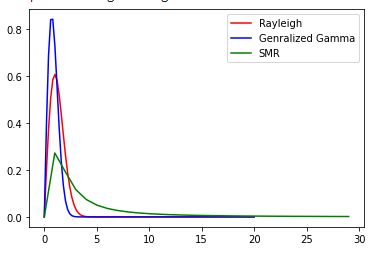
\includegraphics[ width=.8\textwidth , height =5cm]{sim pdf.PNG}
\caption{Python simulted pdf in SMR model for $\sigma = 1$ and q=1 }
\label{Fig:1}
\end{figure}
\end{column}

\end{columns}
The python code for the figure is
\hbox{
https://github.com/Swati-Mohanty/AI5002/blob/main/Project/codes/smr pdf.py}
\end{frame}

\subsection{Plots}
\begin{frame}
\frametitle{Simulated CDF Plots }
\footnotesize
\label{a}
\begin{columns}
\begin{column}{.8\textwidth}
\begin{figure}[h]
\renewcommand{\theenumi}{1}
\centering
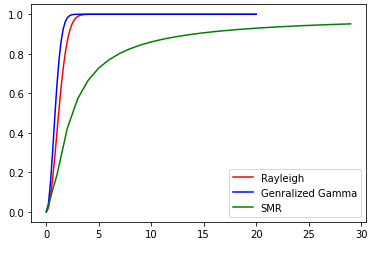
\includegraphics[ width=.8\textwidth , height =5cm]{sim cdf.PNG}
\caption{Python simulated cdf in SMR model for $\sigma = 1$ and q = 1 }
\label{Fig:1}
\end{figure}

\end{column}

\end{columns}
The python code for the figure is
\hbox{
https://github.com/Swati-Mohanty/AI5002/blob/main/Project/codes/smr\_cdf.py}

\end{frame}

\subsection*{Simulation Study}
\begin{frame}[fragile]
\footnotesize
\frametitle{Simulation Study}
The performance of ML estimates for finite sample size were studied to check if the estimators satisfy the desirable properties.
\begin{figure}[h]
\renewcommand{\theenumi}{1}
\centering
\includegraphics[ width=\textwidth , height =5cm]{pp1.PNG}
\caption{Graphics of (a) bias (b) RMSE and (c) coverage of simulator for $\sigma =1 , q = 1 , n = 30...200$ in SMR model }
\label{Fig:1}
\end{figure}

\end{frame}

\subsection*{Simulation Study 2}
\begin{frame}[fragile]
\footnotesize
%\frametitle{Simulation Study}

\begin{figure}[h]
\renewcommand{\theenumi}{1}
\centering
\includegraphics[ width=\textwidth , height =5cm]{pp4.PNG}
\caption{Graphics of (a) bias (b) RMSE and (c) coverage of simulator for $\sigma =10 , q = 1.5 , n = 30...200$ in SMR model }
\label{Fig:1}
\end{figure}
{INFERENCES}
\begin{itemize}
    \item As sample size increases, then bias and RMSE decreases. This suggests that the estimators are consistent.
    \item As sample size increases, the empirical coverage probability approaches to the nominal level (95\%)
\end{itemize}
\end{frame}

\subsection{a}
\begin{frame}
\frametitle{Application 1:Patients with Bladder cancer}
\footnotesize
\label{a}
\begin{columns}
\begin{column}{.6\textwidth}
\begin{figure}[h]
\renewcommand{\theenumi}{1}
\centering
\includegraphics[ width=\textwidth , height =5cm]{pp5.PNG}
\caption{Density plot of patients with bladder cancer in the R, SR and SMR distribution }
\label{Fig:1}
\end{figure}
\end{column}

\begin{column}{.4\textwidth}
\begin{table}[htbp]
\centering
  \resizebox{\textwidth}{!}{\begin{minipage}{\textwidth}
\begin{tabular}{ |p{1cm}|p{2cm}|  }
\hline
 \multicolumn{2}{|c|}{Statistical Values} \\
\hline
n & 128\\
\hline
\overline{T} & 9.366\\
\hline
S & 10.508\\
\hline
$\sqrt{b_1}$ & 3.287\\
\hline
b_2 & 18.483\\
\hline
min(T) & 0.08\\
\hline
max(T) & 79.05\\
\hline
\end{tabular}
\end{minipage}}
\caption{\tiny Descriptive statistics}
\end{table}
\end{column}
\end{columns}
\end{frame}

\subsection{b}
\begin{frame}
\frametitle{Application 1:Patients with Bladder cancer}
\footnotesize
\label{a}
\begin{columns}

\begin{column}{\textwidth}
\begin{figure}[h]
\renewcommand{\theenumi}{1}
\centering
\includegraphics[ width=7cm, height =5cm]{pp6.PNG}
\caption{QQ plot of patients with bladder cancer in the (a)R, (b)SR and (c)SMR distribution }
\label{Fig:2}
\end{figure}
\end{column}
\end{columns}
\end{frame}

\subsection{c}
\begin{frame}
\frametitle{Application 2:Number of failures of an air conditioning system}
\footnotesize
\label{c}
\begin{columns}
\begin{column}{.6\textwidth}
\begin{figure}[h]
\renewcommand{\theenumi}{1}
\centering
\includegraphics[ width=\textwidth , height =5cm]{pp7.PNG}
\caption{Density plot of number of failures of an air conditioning system in the R, SR and SMR distribution }
\label{Fig:1}
\end{figure}
\end{column}

\begin{column}{.4\textwidth}
\begin{table}[htbp]
\centering
  \resizebox{\textwidth}{!}{\begin{minipage}{\textwidth}
\begin{tabular}{ |p{1cm}|p{2cm}|  }
\hline
 \multicolumn{2}{|c|}{Statistical Values} \\
\hline
n & 188\\
\hline
\overline{T} & 92.074\\
\hline
S & 107.916\\
\hline
S & 10.508\\
\hline
$\sqrt{b_1}$ & 2.139\\
\hline
b_2 & 8.023\\
\hline
min(T) & 1\\
\hline
max(T) & 603\\
\hline
\end{tabular}
\end{minipage}}
\caption{\tiny Descriptive statistics}
\end{table}
\end{column}
\end{columns}
\end{frame}

\subsection{d}
\begin{frame}
\frametitle{Application 2:Number of failures of an air conditioning system}
\footnotesize
\label{d}
\begin{columns}

\begin{column}{\textwidth}
\begin{figure}[h]
\renewcommand{\theenumi}{1}
\centering
\includegraphics[ width=7cm , height =5cm]{pp8.PNG}
\caption{QQ plot of number of failures of an air conditioning system in the (a)R, (b)SR and (c)SMR distribution }
\label{Fig:2}
\end{figure}
\end{column}
\end{columns}
\end{frame}

\subsection{e}
\begin{frame}
\frametitle{CONCLUSION}
\footnotesize
\label{e}
\begin{columns}
\column{.8\textwidth}
\setbeamertemplate{itemize items}[square]
  \begin{itemize}
  \item More flexible model as for its kurtosis coefficient and hazard function than the Rayleigh and slashed
Rayleigh distribution.
  \item A simulation study is included, which suggests that the ML
estimators are consistent even for moderate sample sizes
  \item QQ-plots show that our proposal provides a better fit than R and SR distributions,
especially on the right tail of these data sets.
  \end{itemize}
  \end{columns}
\end{frame}

\subsection{d}
\begin{frame}
\frametitle{REFERENCES}
\footnotesize
\label{d}
\ [1.] Siddiqui, M.M. Some problems connected with Rayleigh distributions. J. Res. Natl. Bureu Stand. Ser. D 1962,
66, 167–174. [CrossRef]
\\\ [2.] Miller, K.S. Multidimensional Gaussian Distributions; Wiley: New York, NY, USA, 1964.
\\\ [3.] Polovko, A.M. Fundamentals of Reliability Theory; Academic Press: San Diego, CA, USA, 1968.
\\\ [4.] Hirano, K. Rayleigh distribution, In Encyclopedia of Statistical Sciences; Kotz, S., Johnson, N.L., Read, C.B., Eds.;
Wiley: New York, NY, USA, 1986; pp. 647–649.
\\\ [5.] Lopez-Blazquez, J.F.; Barranco-Chamorro, I.; Moreno-Rebollo, J.L. Umvu estimation for certain family of
exponential distributions. Commun. Stat.-Theory Methods 1997, 26, 469–482. [CrossRef]

\end{frame}



\end{document}
